\documentclass[11pt]{extarticle}
\usepackage[a4paper, total={6in, 8.5in}, top=1in, bottom=1in, left=1in, right=1in]{geometry}

\usepackage{mathtools}
\usepackage{graphicx}
\usepackage{amssymb}
\usepackage{amsmath}
\usepackage{pythonhighlight}
\usepackage{pdfpages}
\usepackage[T1]{fontenc}
\usepackage[utf8]{inputenc}
\usepackage{fancyhdr}
\usepackage{pythonhighlight}
\usepackage{changepage}
\usepackage{slashbox}
\usepackage{floatrow}
\usepackage{listings}
\usepackage[hidelinks]{hyperref}
\usepackage{fontawesome}
\usepackage{subcaption}
\usepackage{color} %red, green, blue, yellow, cyan, magenta, black, white
\definecolor{mygreen}{RGB}{28,172,0} % color values Red, Green, Blue
\definecolor{mylilas}{RGB}{170,55,241}


\floatsetup[table]{capposition=top}

\sloppy
\definecolor{lightgray}{gray}{0.5}
\setlength{\parindent}{0pt}
\setlength{\headheight}{14pt}

\renewcommand{\headrulewidth}{.4mm} % header line width
\newcommand{\norm}[1]{\left\lVert#1\right\rVert}

\pagestyle{fancy}
\fancyhf{}
\fancyhfoffset[L]{-1cm} % left extra length
\fancyhfoffset[R]{-1cm} % right extra length
\rhead{\bfseries Kutay U\u{g}urlu 2232841}
\lhead{EE583 Homework 5}
\rfoot{}

\DeclarePairedDelimiter\ceil{\lceil}{\rceil}
\DeclarePairedDelimiter\floor{\lfloor}{\rfloor}

\author{Kutay U\u{g}urlu 2232841}

\begin{document}

\lstset{language=Matlab,%
    %basicstyle=\color{red},
    breaklines=true,%
    morekeywords={matlab2tikz},
    keywordstyle=\color{blue},%
    morekeywords=[2]{1}, keywordstyle=[2]{\color{black}},
    identifierstyle=\color{black},%
    stringstyle=\color{mylilas},
    commentstyle=\color{mygreen},%
    showstringspaces=false,%without this there will be a symbol in the places where there is a space
    numbers=left,%
    numberstyle={\tiny \color{black}},% size of the numbers
    numbersep=9pt, % this defines how far the numbers are from the text
    emph=[1]{for,end,break},emphstyle=[1]\color{red}, %some words to emphasise
    %emph=[2]{word1,word2}, emphstyle=[2]{style},    
}

\fancyfoot[C]{\thepage}
\title{\LARGE \LARGE EE583 Pattern Recognition HW5}

\maketitle{\LARGE}

\pagebreak


\section{Question 1}

\indent 3 different experiments are conducted. In each experiment, ten models are individually used to calculate the accuracy, or equivalently misclassification loss. 

\subsection{Default settings}
\vspace*{-.5cm}
\begin{center}
    \begin{figure}[h]
        {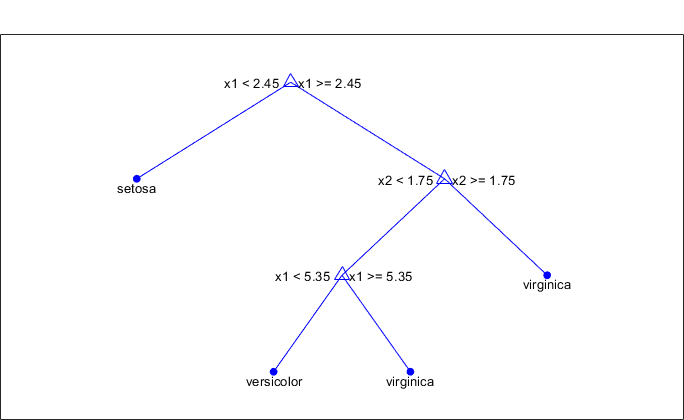
\includegraphics[width = 4in, height = 2.5in]{QT_default.png}}
        \caption{Visualization of the first tree}
        \label{fig:q1_tree}
    \end{figure}
\end{center}
\vspace*{-1cm}
This 3 split tree resulted in a loss of $0.0267$.

\subsection{Maximum number of Splits Restriction}
\vspace*{-.5cm}
\begin{center}
    \begin{figure}[h]
        {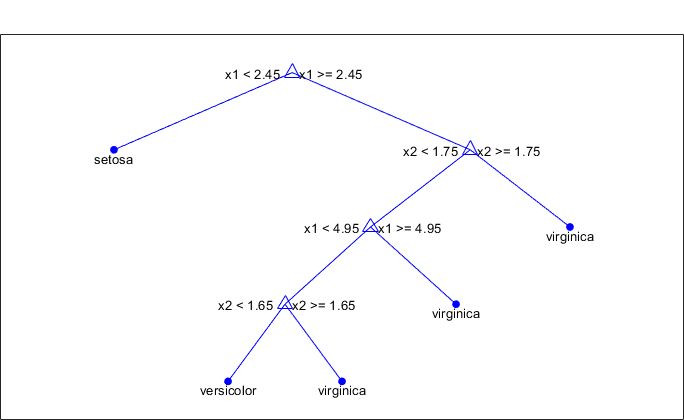
\includegraphics[width = 4in, height = 2.5in]{QT_maxsplit.png}}
        \caption{Visualization of the second tree}
        \label{fig:q1_tree_split}
    \end{figure}
\end{center}
\vspace*{-1cm}
For this experiment the resultant number of splits was higher than the first one. Therefore, it resulted in less misclassification loss of $0.0240$.

\subsection{Maximum number of Splits Restriction}

Changing the split criterion from Gini's diversity index to deviance resulted in the improvement of the accuracy.

\section{Question 2}

\subsection{Single tree vs Ensemble}

To observe the performance difference between a single tree and the ensemble better, the number of splits were set to 1 to decrease the classification capability of the single tree. Otherwise, even the first week learner is able to classify the data accurate enough.\\
\begin{center}
    \begin{minipage}{0.3\textwidth}
        $Accuracy_{first} = 0.64$
        \end{minipage}
        \begin{minipage}{0.3\textwidth}
        $Accuracy_{ensemble} = 0.95$
        \end{minipage}
\end{center}
The results reflect our expectations on the performance of the ensemble trained with Adaboost being better. 
\begin{figure}[h]
    \centering
    {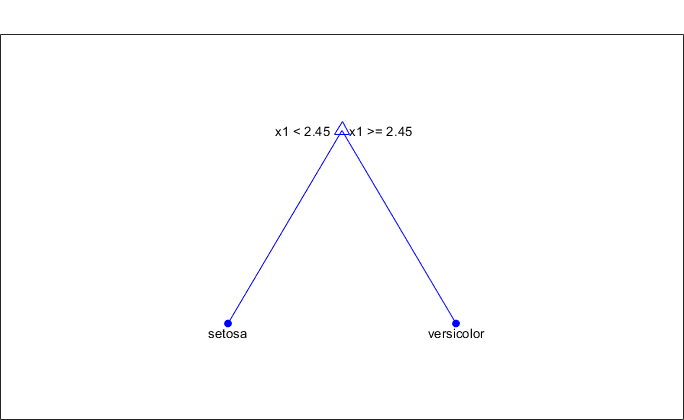
\includegraphics[width = 4in, height = 2.5in]{Q2T.png}}
    \caption{Visualization of the first tree}
    \label{fig:q2_tree}
\end{figure}

\subsection{Learning Rate}
\begin{figure}[h]
    \centering
    {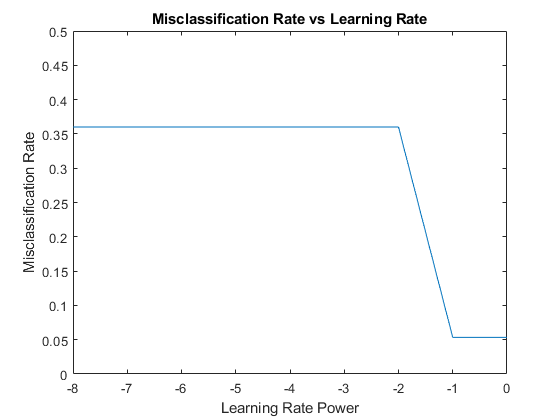
\includegraphics[width = 4in, height = 2.5in]{lr.png}}
    \caption{Learning Rate vs Misclassification}
    \label{fig:q2_lr}
\end{figure}

Again, the maximum number of splits is fixed among experiments, which can be seen in \ref{subsec:Q2_code}. Larger learning rates resulted ensemble to achieve higher accuracy, since the informative samples have more weights in the training process.

\section{Question 3}
\subsection{Learning Rate}
\begin{figure}[h]
    \centering
    {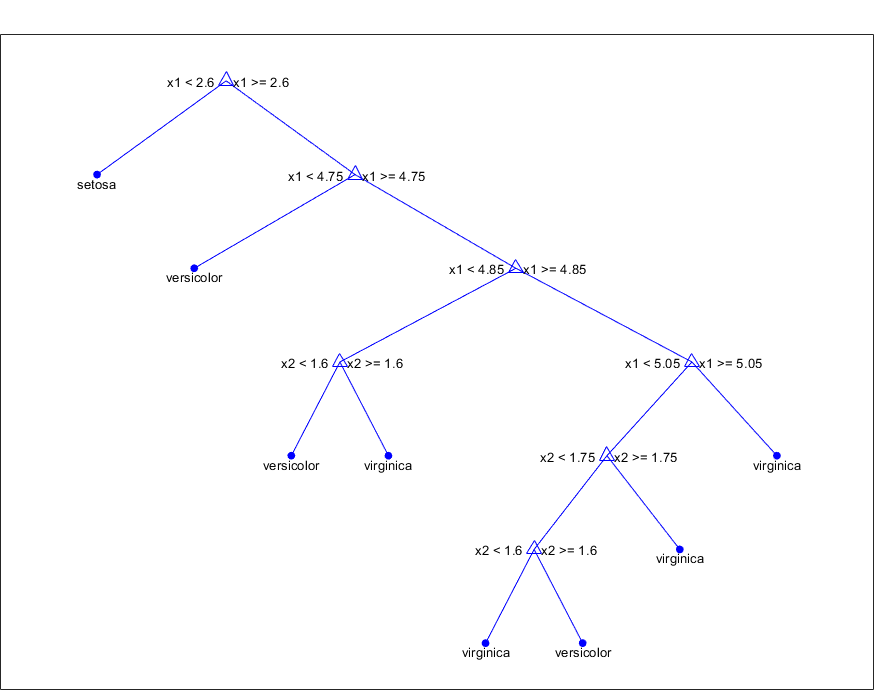
\includegraphics[width = 4in, height = 2.5in]{Q3tree.png}}
    \caption{First Tree}
    \label{fig:q3_tr}
\end{figure}

The accuracy of the first tree is calculated as $0.9867$ whereas the forest's is 1. We see that, with the help of the 24 remaining tree models in the treebagger object, the model was able to classify the samples correctly that are misclassified by the first tree. Hence, the classification accuracy improved. 

\section{Question 4}


\begin{figure}[h]
    \centering
    \begin{subfigure}{4cm}
        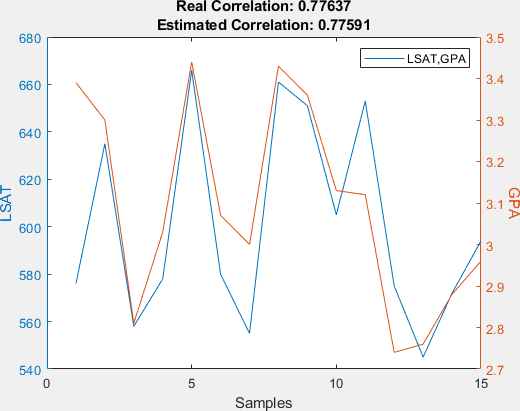
\includegraphics[width=\linewidth]{Q4_2.png}
        \caption{Correlation Estimate}\label{fig:q4a}
    \end{subfigure}
    \qquad
    \begin{subfigure}{4cm}
        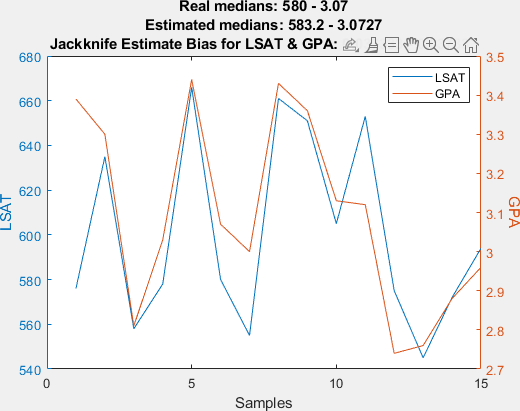
\includegraphics[width=4cm]{Q4_1.png}
        \caption{Median Estimate}\label{fig:q4b}
    \end{subfigure}
    \caption{Jackknife estimates}%
    \label{fig:q4}%
\end{figure}

The variables are plotted with respect to different axes in both Figure \ref{fig:q4a} and \ref{fig:q4b}. The estimates and the estimated bias are calculated and printed in the title. The resultant biases are respectively low when the variance of the relative variables are taken into account.

\pagebreak
\section{APPENDIX}
The code given in this section is shared \href{https://github.com/kutay-ugurlu/Pattern-Recognition/tree/master/HW5}{@\faGithubSquare}.
\subsection{Q1}\label{subsec:Q1_code}
\lstinputlisting{HW5_Q1.m}
\pagebreak
\subsection{Q2} \label{subsec:Q2_code}
\lstinputlisting{HW5_Q2.m}
\pagebreak
\subsection{Q3}\label{subsec:Q3_code}
\lstinputlisting{HW5_Q3.m}
\pagebreak
\subsection{Q4}\label{subsec:Q4_code}
\lstinputlisting{HW5_Q4.m}
\end{document}